% begin module EVT-hypotheses
\begin{frame}[t]
\begin{theorem}[The Extreme Value Theorem]
If \alert<3-4>{$f$ is continuous} on a \alert<5-6>{closed interval $[a,b]$}, then $f$ attains its absolute maximum value $f(c)$ and its absolute minimum value $f(d)$ at some numbers $c$ and $d$ in $[a,b]$.
\end{theorem}
\begin{columns}[c]
\column{.5\textwidth}
\ \uncover<3->{%
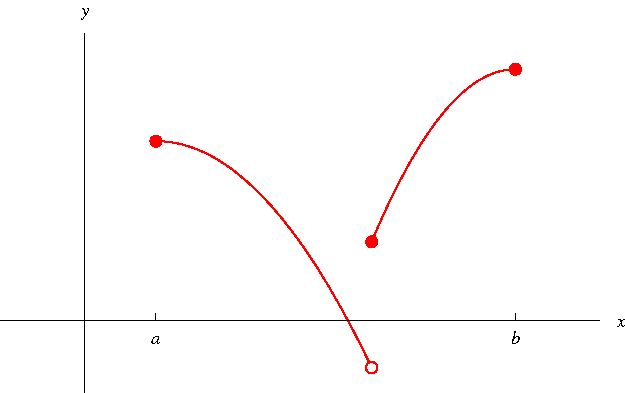
\includegraphics[width=6cm]{maxima-minima/pictures/04-01-evtcounterb.pdf}%
}%
\column{.5\textwidth}
\ \uncover<5->{%
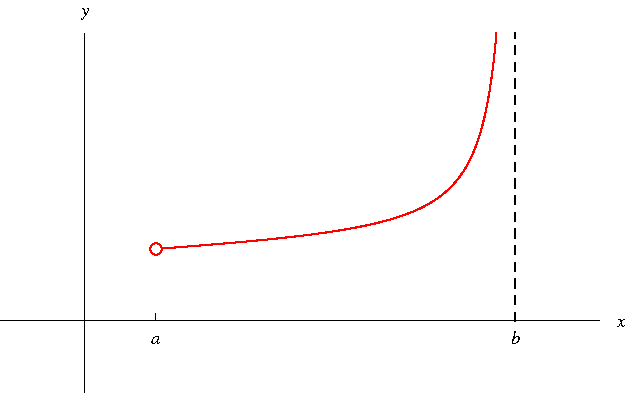
\includegraphics[width=6cm]{maxima-minima/pictures/04-01-evtcountera.pdf}%
}%
\end{columns}
\begin{itemize}
\item  Do we need all of the hypotheses of the theorem?
\item<2-| alert@3-4>  Do we need $f$ to be continuous?  \uncover<4->{Yes.}
\item<2-| alert@5-6>  Do we need the interval to be closed?  \uncover<6->{Yes.}
\end{itemize}
\end{frame}
% end module EVT-hypotheses
